\section{Example Run}
This section presents some screenshots of a full run of the system in a couple configuration.

\begin{figure}[htb]
		\center
		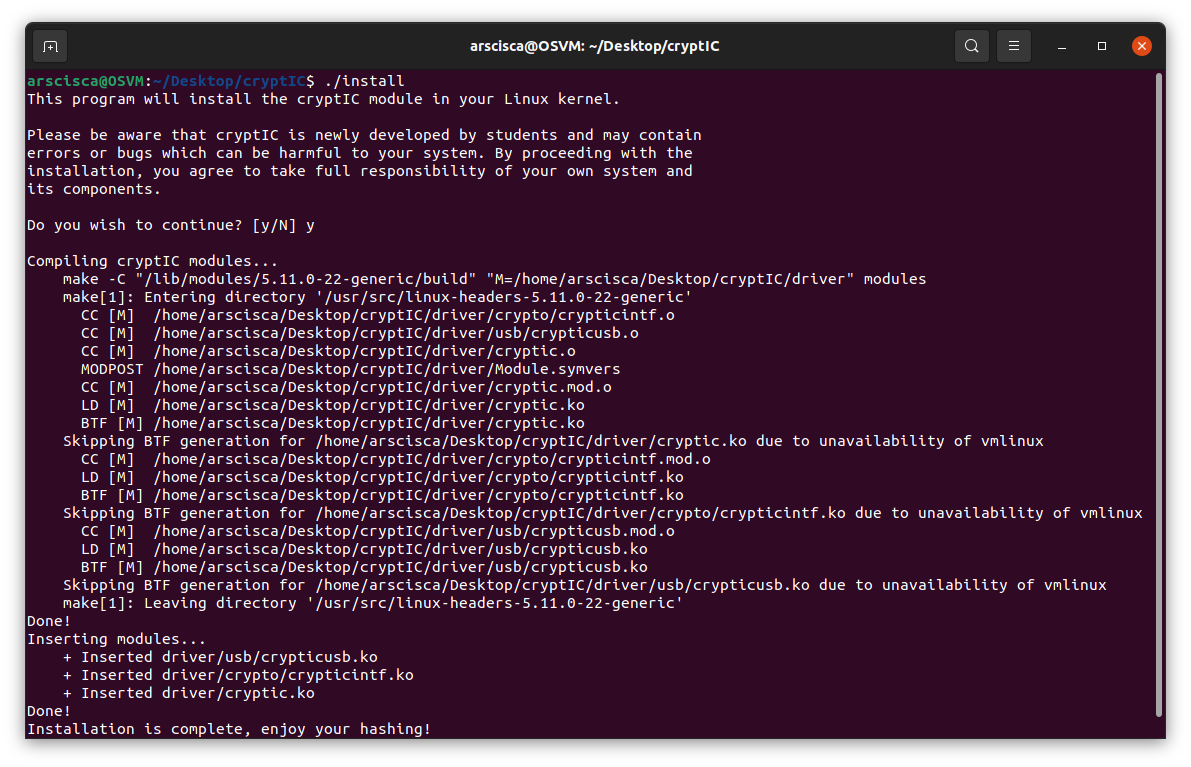
\includegraphics[width=\textwidth]{img/install.png}
		\caption{Driver installation}
\end{figure}

\begin{figure}[htb]
		\center
		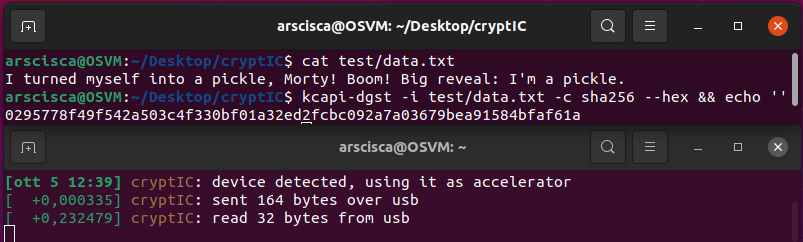
\includegraphics[width=\textwidth]{img/hash_device.png}
		\caption{Hashing example (with device connected)}
    \label{img:hash_dev}
\end{figure}
\begin{figure}[htb]
		\center
		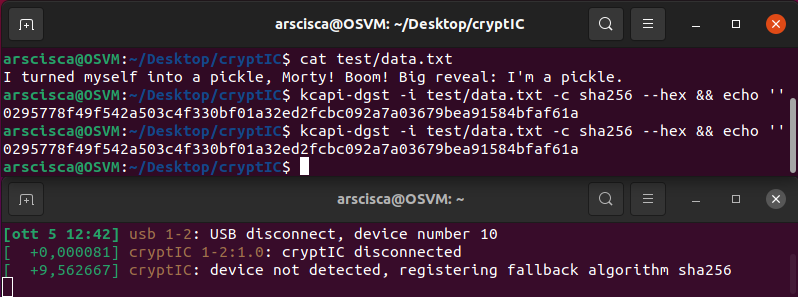
\includegraphics[width=\textwidth]{img/hash_nodev.png}
		\caption{Hashing example (with device disconnected)}
    \label{img:hash_nodev}
\end{figure}
\autoref{img:hash_dev} and \autoref{img:hash_nodev} are particularly interesting because they show the driver in action when using an external command - to show its natural integration with the system - and its seamless operation regardless of whether the device is currently connected or not. In the former case the device actively takes part in the hashing process, in the latter the fallback function is triggered so that no interruption to the user.


\begin{figure}[htb]
		\center
		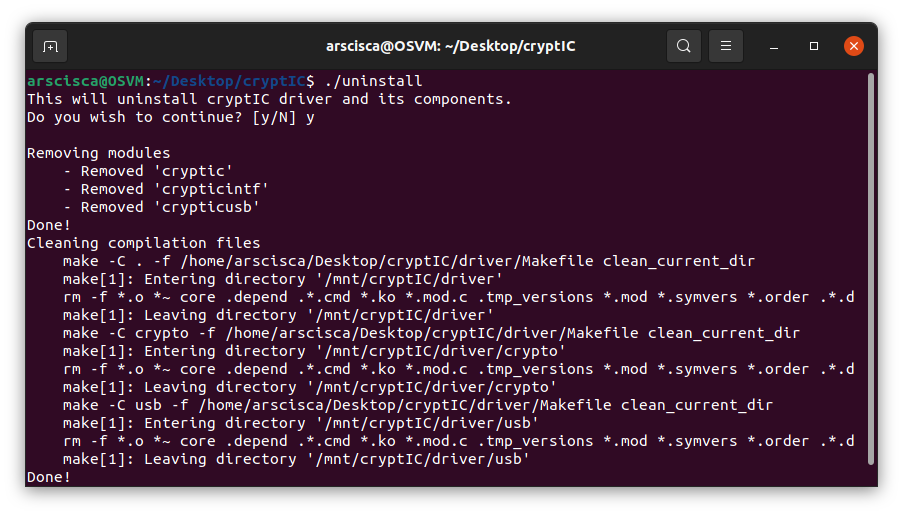
\includegraphics[width=\textwidth]{img/uninstall.png}
		\caption{Uninstalling the driver}
\end{figure}
